\section{How the efficiency is defined}\label{app:effdef}
\intent{The one definition behind every efficiency in the paper, and the choice of the matching radius, with the two
figures that support it (Dylan 2026-11-03: moved out of \cref{sec:detected}).}

\textbf{Denominator.} One reference ray per event: a clean M3 track ($\chi^2<1$, four clusters), decoder-complete
events only, whose footprint at the chamber lies inside the measured active area. The headline numbers use the whole
active area; the interior (${\ge}30$\,mm from the $x$ sides, ${\ge}8$\,mm from the $y$ sides) is quoted where the angle
is involved, and \cref{fig:effradius,fig:residuals} are drawn on the interior. Nothing else leaves the denominator:
tracks whose reference may be bent, edge effects, discharges, $\delta$-rays and second particles we cannot separate
count as losses. Only a second particle shown to be independent of the muon (separate in both views, charge-paired) leaves
the single-track sample, and then the event is counted in the two-particle table, not dropped (\cref{sec:detected}).

\textbf{Numerator: any candidate.} The reconstruction returns several track candidates per view when the event has
more than one deposit. A muon is counted as found when, in each view, the candidate nearest to the reference ray, whatever
rank the reconstruction gave it, is within $R$ of it, with $|r|=\sqrt{\Delta x^2+\Delta y^2}\le R$ at the mesh
(\texttt{budget.py:174,189--190}, \texttt{single\_track\_area.py:87}: detected, or the nearest-candidate match in both
views; the fitted candidates are the sane ones, $|\tan\theta|$ and $p_0$ inside the plate). If the reconstruction keeps the
wrong one of two tracks and the other matches the muon, the event is therefore efficient. This is the multi-track credit
and every quoted efficiency uses it (full area: 94.2\,\% all rays, 94.8\,\% single tracks; interior single tracks 95.7\,\%).
The stricter count, in which only the track the reconstruction keeps may match and both views need at most two competing
strips, is the production pick (91.5\,\% over the full area); it is not drawn here because it measures the track selection
as well as the chamber, and the selection is a separate question (\cref{sec:pairing}). One limit: the nearest candidates of
the two views are chosen independently, so the credit does not check that they are the same particle; the pairing of X and
Y is studied on its own in \cref{sec:pairing}.

\textbf{The radius.} $\varepsilon(R)$ (\cref{fig:effradius}) has two regimes: the resolution core, steep up to
${\sim}4$\,mm, then a slow rise of 0.1--0.2\,pt per mm out to 40\,mm. We use $R=5$\,mm, the knee, where the accidental rate
is 0.07\,\%, below the statistical error and 70$\times$ below the inefficiency; $R\in[4,8]$\,mm moves the efficiency by
$-0.5/{+0.7}$\,pt on the single-track efficiency (the systematic quoted in \cref{sec:detected}; the all-rays curve of \cref{fig:effradius} moves by $-0.5/{+0.7}$). The accidental curve is the probability that an unrelated track lands inside $R$: the
chamber's fit of one event is compared with the reference ray of another event (event mixing, 20 shifts), scaled by the
fraction of events with a fit. It is an upper bound on fakes, since in a real event the muon is also there.

\begin{figure}[tbp]
  \centering
  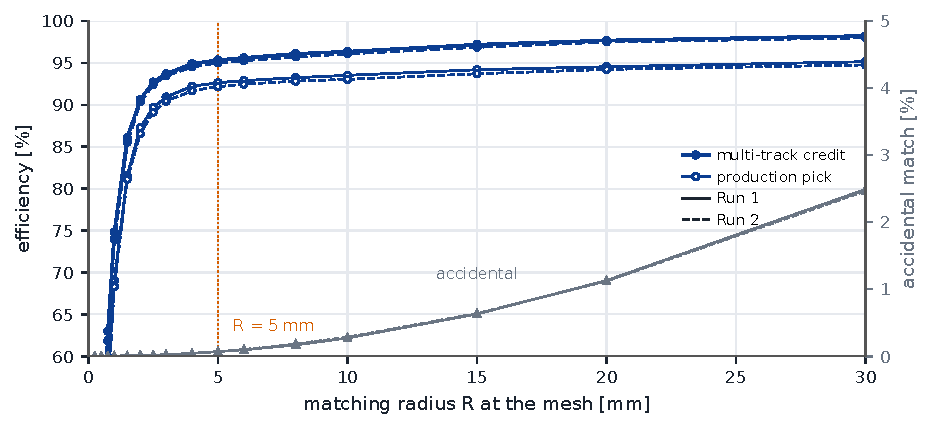
\includegraphics[width=\linewidth]{eff_vs_radius}
  \caption{Chamber~A efficiency (Runs 1 and 2 combined, interior) against the matching radius $R$ at the mesh. The muon counts as found if any reconstructed track candidate lies within $R$ of the reference ray (95.1\,\% at $R=5$\,mm). Grey, right axis: the probability that an unrelated track (the chamber's fit of another event) falls within $R$ of a given reference ray. Dotted: $R=5$\,mm.}
  \label{fig:effradius}
\end{figure}

\textbf{Why 5\,mm and not a few $\sigma$ of the resolution.} The residual at the mesh is not the chamber's
resolution: a Gaussian fit to its core (\cref{fig:residuals}a, $|r|<1.5$\,mm) gives $\sigma=0.55\pm0.02$ (X) and
$0.53\pm0.03$\,mm (Y), of which the chamber contributes ${\sim}0.12$\,mm (\cref{sec:posres}); the rest is the reference
pointing at the chamber (0.24/0.21\,mm) and the multiple scattering of soft cosmic muons. Its tails are not Gaussian:
only 94/92\,\% (X/Y) of the fitted tracks lie within 3$\sigma$ of the reference, 98\,\% within 5\,mm. A cut at
3$\sigma$ (${\approx}1.6$\,mm) would count 11\,pt of tracks the chamber did find, on the right particle, as losses,
mixing the reference's resolution tails into the efficiency. The efficiency asks whether the chamber saw the muon;
how well it measured it is the resolution (\cref{sec:tracking}). Between 1.6 and 5\,mm the efficiency rises by 11\,pt
while the accidental rate stays below 0.07\,\%, so those tracks are the muon, measured less well.

\textbf{What lies beyond 5\,mm} (\cref{fig:residuals}b). The grey curve is the distance to another event's reference
ray, scaled as if every fit were unrelated to its muon: an unrelated fit lands mostly ${>}40$\,mm away. The data have
7 tracks there against 16\,300 for that hypothesis, so at most ${\sim}0.05$\,\% of fits are unrelated, and they
contribute ${<}1$ of the 244 tracks at 10--20\,mm. The shoulder from 5 to 20\,mm is therefore correlated with the
muon: fits pulled by its $\delta$-rays and saturated blobs, a secondary fitted instead of the muon, and bent reference tracks
(the classes of \cref{app:losses}). We cut before it, and count what lies beyond as loss. The residual distributions are
those of the track the reconstruction keeps (both views fitted, no radius cut), so they show what the production pick
measures, not the any-candidate count.

\begin{figure}[tbp]
  \centering
  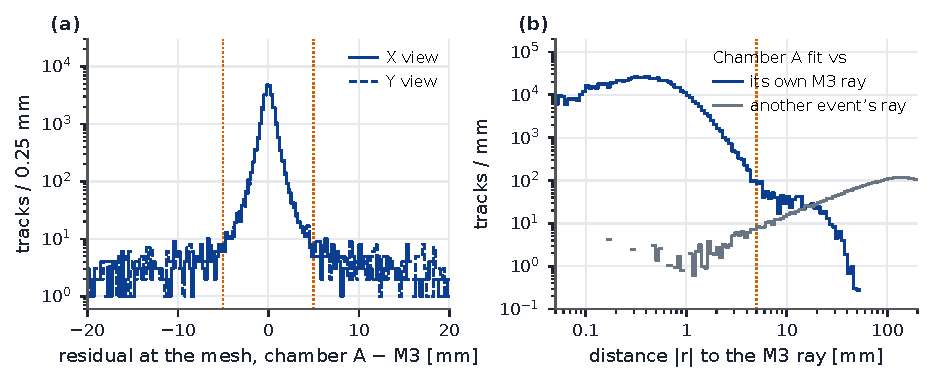
\includegraphics[width=\linewidth]{residuals}
  \caption{The full chamber~A residual distributions behind \cref{fig:effradius}, Runs 1 and 2 summed: (a) per view at the mesh (0.25\,mm bins; X blue solid, Y orange dashed), (b) radial, with the distance to another event's ray (event mixing, scaled to the same number of fits: what the data would be if every fit were unrelated to its muon). Black in (a): a Gaussian fit to the core ($|r|<1.5$\,mm), $\sigma=0.55$ (X) / 0.53\,mm (Y). Dotted: $R=5$\,mm. The 5--20\,mm shoulder is correlated with the muon, not accidental: the data have 7 tracks beyond 40\,mm where unrelated fits would put 16\,300.}
  \label{fig:residuals}
\end{figure}
